\documentclass{article}

\usepackage{graphicx}
\usepackage{tikz}
\usepackage{tikzsymbols}
\usetikzlibrary{calc,patterns,shapes.geometric}
\pagestyle{empty}
\usepackage[margin=0pt]{geometry}
\geometry{papersize={14in,12in}}

\def\centerarc[#1](#2)(#3:#4:#5){\draw[#1] ($(#2)+({#5*cos(#3)},{#5*sin(#3)})$) arc (#3:#4:#5);}

\begin{document}
	\begin{figure}
		\centering
		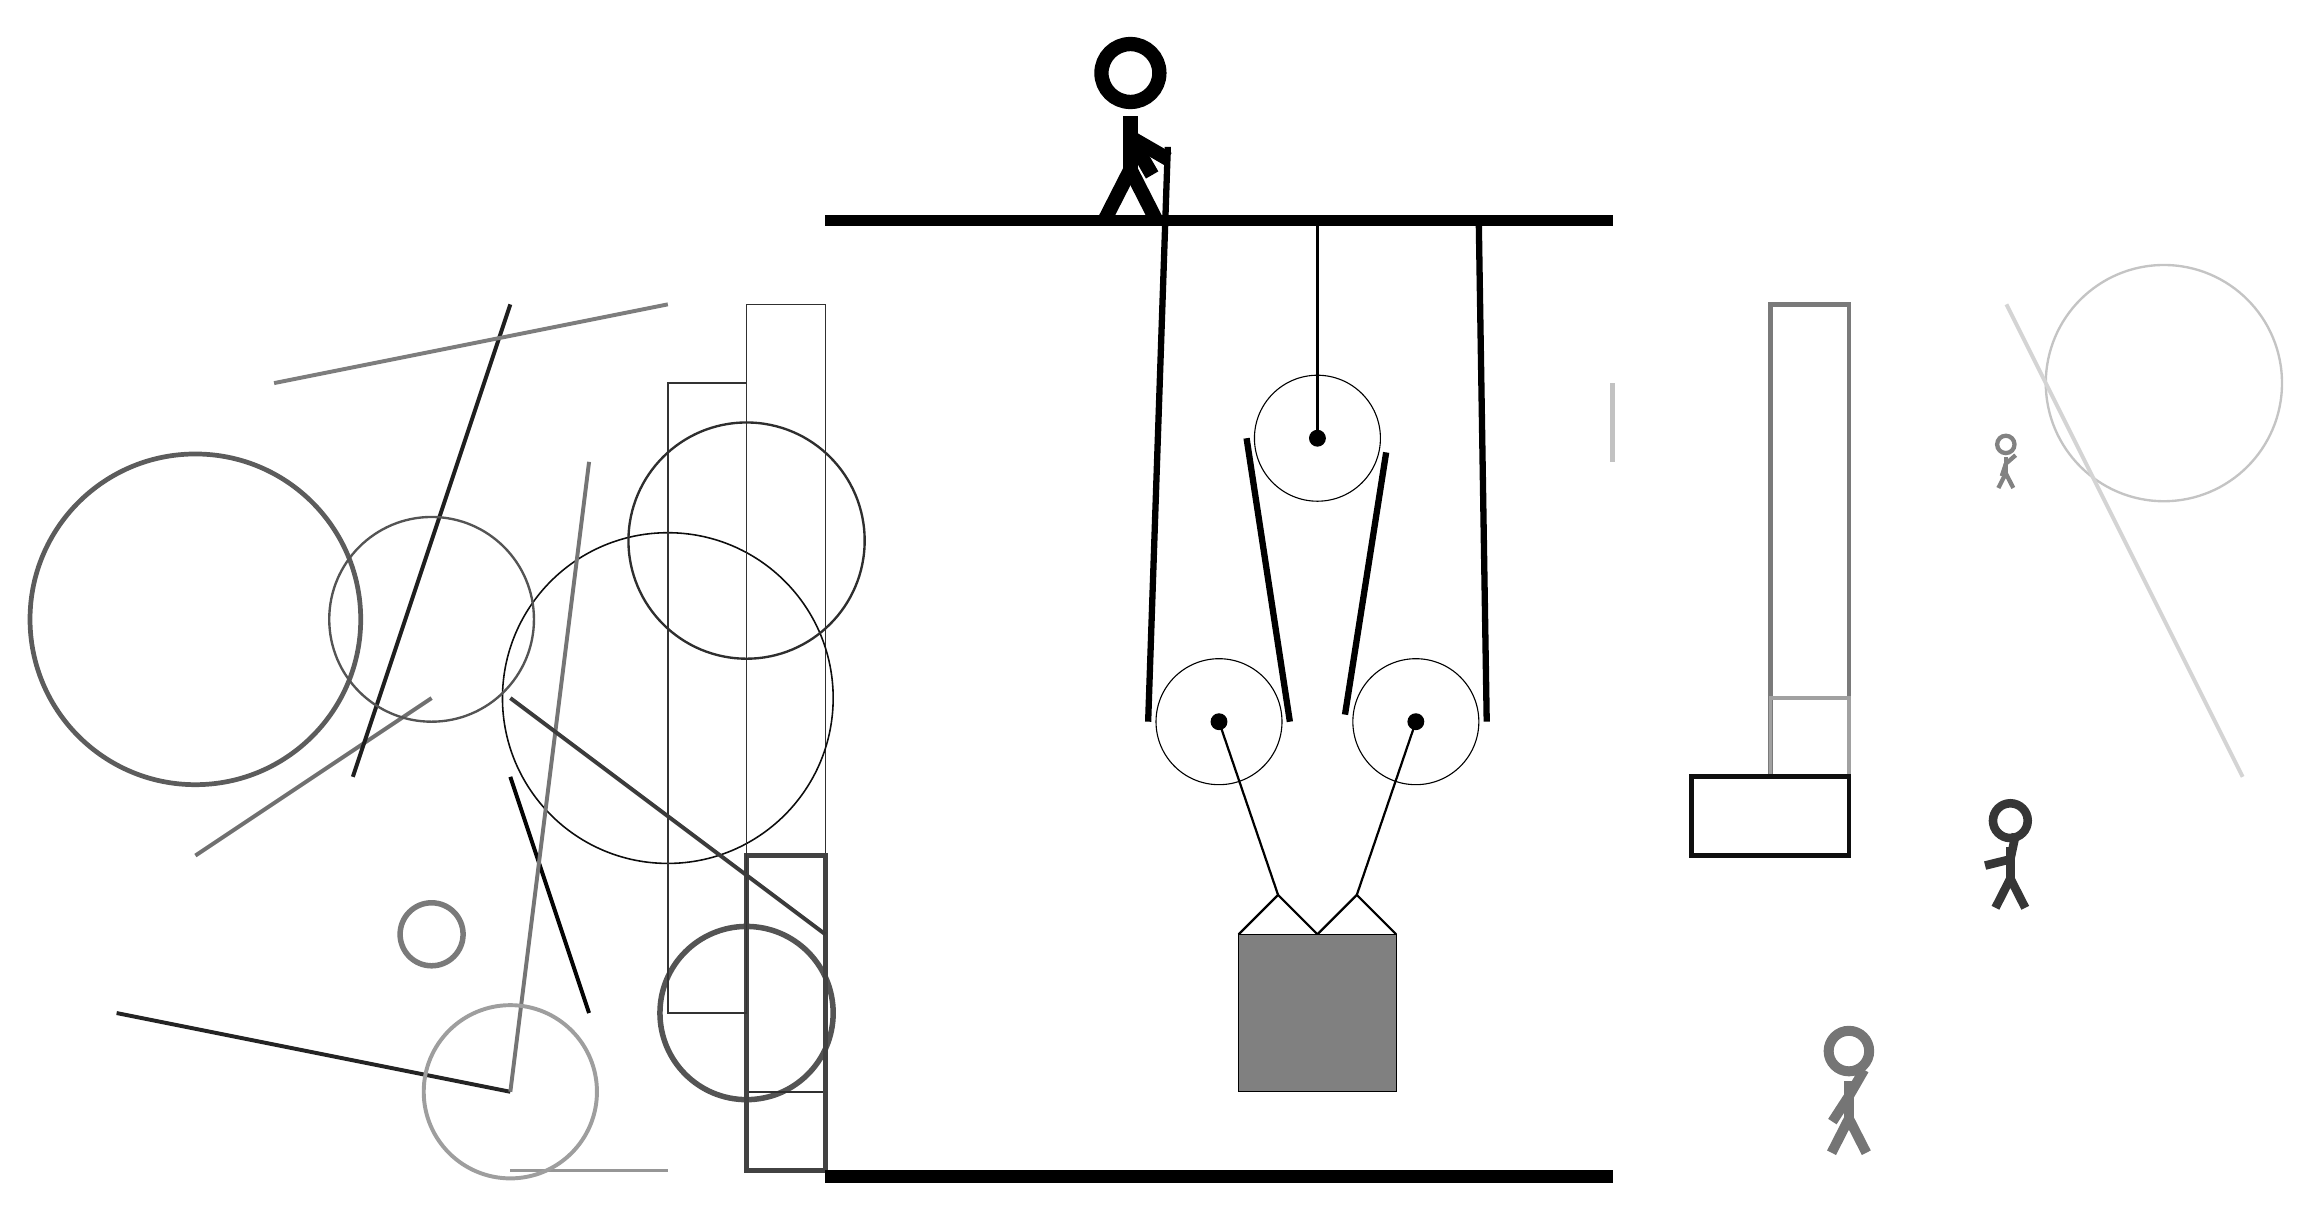
\begin{tikzpicture}
			%%%%% START %%%%%
			
			\draw[fill=black] (-4, 9) rectangle (6, 9.125);
			
			\draw[line width=0.5mm, color=black!56](-9, 3) -- (-12, 1);
			
			\draw [line width=0.7mm, color=black!67](-5, -1) circle (1.1);
			\draw[line width=0.5mm, color=black!41](-6, -3) -- (-8, -3);
			\draw[line width=0.2mm, color=black!81] (-5, -2) rectangle (-4, 8);
			\draw [line width=0.6mm, color=black!64](-12, 4) circle (2.1);
			\draw [line width=0.2mm, color=black!95](-6, 3) circle (2.1);
			\draw[line width=0.6mm, color=black!24] (6, 6) rectangle (6, 7);
			\draw[line width=0.6mm, color=black!74] (-5, 1) rectangle (-4, -3);
			\node[line width=0.6mm, color=black!79] at (11, 1) {\Strichmaxerl[6][14][78]};
			\draw[line width=0.5mm, color=black!88](-8, 8) -- (-10, 2);
			\draw[line width=0.5mm, color=black!86](-8, -2) -- (-13, -1);
			
			\node[line width=0.2mm, color=black!49] at (11, 6) {\Strichmaxerl[3][72][41]};
			\draw[line width=0.6mm, color=black!52] (8, 2) rectangle (9, 8);
			\draw [line width=0.3mm, color=black!23](13, 7) circle (1.5);
			\draw[line width=0.5mm, color=black!17](11, 8) -- (14, 2);
			\draw[line width=0.5mm, color=black!98](-8, 2) -- (-7, -1);
			
			\draw[line width=0.4mm, color=black!37] (8, 3) rectangle (9, 2);
			\draw[line width=0.6mm, color=black!94] (7, 1) rectangle (9, 2);
			\draw[line width=0.2mm, color=black!80] (-6, 7) rectangle (-5, -1);
			\draw [line width=0.3mm, color=black!82](-5, 5) circle (1.5);
			\draw [line width=0.3mm, color=black!67](-9, 4) circle (1.3);
			
			\draw[line width=0.5mm, color=black!54](-8, -2) -- (-7, 6);
			\draw[line width=0.5mm, color=black!51](-6, 8) -- (-11, 7);
			\node[line width=0.4mm, color=black!54] at (9, -2) {\Strichmaxerl[7][57][60]};
			\draw[line width=0.5mm, color=black!77](-8, 3) -- (-4, 0);
			\draw [line width=0.7mm, color=black!52](-9, 0) circle (0.4);
			
			\draw [line width=0.5mm, color=black!38](-8, -2) circle (1.1);
			
			\draw (1, 2.7) circle (0.8);
			\draw[fill=black] (1, 2.7) circle (0.1);
			
			\draw (2.25, 6.3) circle (0.8);
			\draw[fill=black] (2.25, 6.3) circle (0.1);
			\draw[thick] (2.25, 6.3) -- (2.25, 9);
			
			\draw (3.5, 2.7) circle (0.8);
			\draw[fill=black] (3.5, 2.7) circle (0.1);
			
			\draw[thick] (3.5, 2.7) -- (2.75, 0.5);
			\draw[thick] (1, 2.7) -- (1.75, 0.5);
			\draw[thick]  (1.25, 0) -- (1.75, 0.5) -- (2.25, 0);
			\draw[thick]  (2.25, 0) -- (2.75, 0.5) -- (3.25, 0);
			\draw[fill=black!50] (1.25, 0) rectangle (3.25, -2);
			
			\draw[line width=0.8mm] (0.35, 10) --  (0.1, 2.7);
			\centerarc[line width=0.8mm](1, 2.7)(180:360:0.9);
			\draw[line width=0.8mm] (1.9, 2.7) -- (1.35, 6.3);
			\centerarc[line width=0.8mm](2.25, 6.3)(-20:180:0.9);
			\draw[line width=0.8mm](3.123, 6.12) -- (2.6, 2.79);
			\centerarc[line width=0.8mm](3.5, 2.7)(160:360:0.9);
			\draw[line width=0.8mm](4.4, 2.7) -- (4.3, 9);
			
			\node at (-0.07, 10.2) {\Strichmaxerl[10][120][-30]};
			
			\draw[fill=black] (-4, -3) rectangle (6, -3.15);
			
			%%%%% END %%%%%
		\end{tikzpicture}
	\end{figure}	
\end{document}